\documentclass[man]{apa7}

\usepackage[american]{babel}
\usepackage{csquotes}
\usepackage{amsmath}
\usepackage{amssymb}
\usepackage{booktabs}
\usepackage{longtable}
\usepackage{array}
\usepackage{microtype}
\usepackage{hyperref}
\usepackage{tikz}
\usetikzlibrary{arrows.meta,positioning,shapes.geometric}
\usepackage[style=apa,sortcites=true,sorting=nyt,backend=biber]{biblatex}

\addbibresource{references.bib}

\title{ARC-ADHD: A Closed-Loop Serious Game Framework for Training Executive Control and Emotion-Regulation Recovery in Children With ADHD}
\shorttitle{ARC-ADHD Closed-Loop Framework}
\authorsnames{Mateusz Pomianek}
\authorsaffiliations{{Department of Computer Science and Automation, Rzeszów University of Technology, Rzeszów, Poland}}
\keywords{ADHD, serious games, emotion regulation, executive functions, closed-loop adaptation, digital health, recovery}

\abstract{Digital serious games for children with attention-deficit/hyperactivity disorder (ADHD) can improve selected trained attention and executive-function outcomes, but clinically meaningful transfer beyond the trained task remains a central challenge. ARC-ADHD is proposed as a closed-loop serious-game framework in which controlled executive challenge is followed by an explicit pause, orientation to current bodily or task state, strategy selection, regulation, recovery monitoring, and return to the interrupted goal. The core intervention deliberately excludes augmented-reality transfer experiments, facial-behavior feedback, bilateral auditory stimulation, and wearable EEG acquisition, which are assigned to separate companion studies or measurement tracks. The principal mechanistic quantity is monitoring-anchored recovery latency \(T_{\mathrm{rec}}\). Recovery is operationalized against a stable target-rule calibration reference using a small preregistered behavioral/timing feature space and a persistence criterion; the immediate preswitch window is used for challenge eligibility rather than as the recovery normalization baseline. Phase 0 first tests recovery-measure validity through prespecified computability, scale, timing-coverage, and perturbation-stability gates before the selected definition is used inferentially. The paper then distinguishes proximal mechanism change, independent near transfer, and externally assessed far transfer, with candidate-specific event denominators and explicit right-censoring. The staged programme comprises co-design and construct validation, feasibility testing, a pilot randomized trial intended to estimate design parameters rather than establish efficacy, and a later confirmatory trial. EDI Reactivity is the leading provisional external endpoint candidate for Phase 1/2 planning, while the confirmatory endpoint remains unfrozen pending a defensible Polish localization and validation pathway. ARC-ADHD is presented as a falsifiable and reproducible computational research framework rather than an established treatment or a completed randomized-trial protocol.}



\hypersetup{
  pdftitle={ARC-ADHD: A Closed-Loop Serious Game Framework},
  pdfauthor={Mateusz Pomianek},
  pdfsubject={Executive control and emotion-regulation recovery in ADHD},
  pdfkeywords={ADHD, serious games, executive function, emotion regulation}
}

\begin{document}
\maketitle

\section{Introduction}

Attention-deficit/hyperactivity disorder (ADHD) is characterized by persistent inattention and/or hyperactivity-impulsivity associated with functional impairment. Difficulties in executive control, persistence after error, frustration tolerance, and emotion regulation are also common in affected children, although emotion dysregulation is not itself a defining diagnostic criterion \parencite{graziano2016dysregulation,wolraich2019guideline}.

Digital interventions provide a useful experimental substrate because task contingencies, challenge intensity, sensory cues, and response timing can be standardized and logged. Randomized trials and reviews show that game-based and computerized interventions can improve selected trained or near-transfer outcomes in pediatric ADHD \parencite{kollins2020stars,oh2024dtx,lin2025seriousgames,yan2026ceft}. EndeavorRx, evaluated in the STARS-ADHD programme, is an important example that digital game-like delivery can support a regulated therapeutic product, but improvement on a targeted attention measure does not by itself establish broad transfer to everyday emotional or functional outcomes \parencite{kollins2020stars}.

The central problem addressed here is therefore not whether a child can become better at a game. It is whether a digital intervention can repeatedly train a measurable transition from challenge back to goal-directed behavior, and whether change in that transition is associated with independent outcomes outside the trained task.

ARC-ADHD treats regulation as a control problem. The child encounters a bounded challenge, interrupts an ineffective response, identifies relevant task or body information, selects a strategy, regulates, and resumes the original goal. Error, frustration, or temporary destabilization are not defined as intervention failure. The key event is successful recovery.

The present paper has two purposes. First, it formalizes the core ARC-ADHD mechanism and its observable quantities as an implementable computational research architecture. Second, it defines a staged evaluation programme that can falsify the central claim before a confirmatory efficacy trial is attempted. It is intentionally not presented as a completed randomized-trial protocol. A future confirmatory protocol should be written after the intervention version, primary endpoint, recovery parameters, active control, and analysis rules have been frozen, and should follow the then-current SPIRIT guidance \parencite{chan2025spirit}.

The computational contribution is fourfold. First, the intervention is represented as a versioned closed-loop state sequence with explicit challenge eligibility, regulation transitions, recovery monitoring, and return-to-goal states. Second, recovery is represented as a reconstructable event-level time-to-event quantity with target-rule-matched normalization, persistence, and right-censoring rather than a single postchallenge score. Third, the measurement context is locked while recovery is assessed so adaptive changes, safety interventions, telemetry loss, ordinary censoring, and scientifically invalid events remain distinguishable. Fourth, the framework couples this measurement contract to deterministic controller replay, versioned telemetry, and explicit BYOD qualification so the delivered intervention and derived recovery records can be reconstructed from the study archive.

Four technology-specific lines have been removed from the principal causal claim. Facial-behavior feedback, bilateral auditory stimulation, embodied/augmented-reality context transfer, and wearable EEG measurement are developed as separate companion papers. This separation reduces scope creep and prevents a null or positive result for one optional technology from being conflated with evidence about the core regulation mechanism.

\section{Scope and Related Work}

\subsection{Digital therapeutics and serious games for ADHD}

The STARS-ADHD trial and subsequent reviews support continued study of digital and game-based interventions in pediatric ADHD while also showing heterogeneity in intervention content, comparators, outcomes, and evidence for generalization \parencite{kollins2020stars,oh2024dtx,lin2025seriousgames,schultz2025content,tommasi2026serious}. ARC-ADHD therefore treats digital delivery as a means of delivering controlled practice, not as evidence of therapeutic efficacy by itself.

\subsection{Emotion regulation as a distinct target}

Emotion dysregulation is associated with ADHD and functional burden \parencite{graziano2016dysregulation}. Psychosocial interventions addressing dysregulation are heterogeneous, and executive-control training cannot be assumed to produce emotion-regulation change merely because both involve control processes \parencite{vacher2020psychosocial,groves2022emotion}. The present model therefore requires an independently assessed emotion-regulation or dysregulation outcome in addition to in-game performance.

\subsection{Why recovery is treated as a temporal target}

Emotion regulation is not only a static level of distress, strategy endorsement, or informant-rated difficulty. Developmental emotion research also characterizes within-person temporal dynamics, including intensity, variability, instability, inertia, and change over time \parencite{reitsema2022emotiondynamics}. In developmental psychobiology, structured self-regulation paradigms explicitly distinguish baseline, challenge reactivity, within-task change, and post-challenge recovery as different temporal contexts \parencite{davis2020context}. This provides a theoretical rationale for making return to goal-directed behavior after a controlled perturbation the central proximal quantity in ARC-ADHD.

This rationale does not establish \(T_{\mathrm{rec}}\) as a validated clinical measure. A recent systematic review of behavioral and physiological emotion-regulation assessment in children and adolescents found substantial heterogeneity in definitions, theoretical embedding, and psychometric reporting, including limited reporting of validity evidence \parencite{bunz2026ermeasurement}. ARC-ADHD therefore treats recovery latency as a project-specific mechanistic measure whose construction, stability, sensitivity to missingness, challenge dependence, and relation to independent outcomes must be established empirically before strong inference.

\subsection{Why the core paper is deliberately narrow}

Earlier versions of ARC-ADHD combined multisensory cueing, sensorimotor synchronization, body awareness, augmented reality, facial behavior, and bilateral audio in a single framework. Such modularity is useful for product design but problematic for causal inference because each component creates distinct mechanisms, measurement error, safety constraints, and statistical contrasts.

The revised programme retains only components required to instantiate the challenge-regulation-recovery cycle in the core paper. Visual, auditory, and haptic cues may be used as bounded information channels, and a brief body-orientation step may be used to connect strategy selection with subjective state. Stronger claims about movement, sensorimotor synchronization, spatial context, and augmented reality are reserved for the embodied/AR companion study. Camera-derived facial behavior and bilateral auditory stimulation are fully outside the core intervention claim. Wearable EEG, including the Muse S Athena companion study, is likewise an optional measurement layer and is not required to define, deliver, or validate the core recovery event.

\subsection{Replicability of a complex behavioral intervention}

The intervention should be described using the TIDieR framework so that rationale, materials, procedures, provider role, delivery mode, setting, dose, tailoring, modifications, and fidelity can be reconstructed \parencite{hoffmann2014tidier}. A later randomized-trial protocol should additionally follow SPIRIT 2025 \parencite{chan2025spirit}. This paper instead defines the mechanism and the development gates that must be completed before such a protocol is credible.

\section{Mechanistic Model}

\subsection{Central regulation cycle}

The core unit of ARC-ADHD is shown in Figure~\ref{fig:closed-loop} and can be summarized as

\[
\begin{gathered}
\text{challenge}
\rightarrow
\text{destabilization}
\rightarrow
\text{pause}
\rightarrow
\text{orient}\\
\rightarrow
\text{select strategy}
\rightarrow
\text{regulate}
\rightarrow
\text{recover}
\rightarrow
\text{resume goal}.
\end{gathered}
\]

\begin{figure}[htbp]
\centering
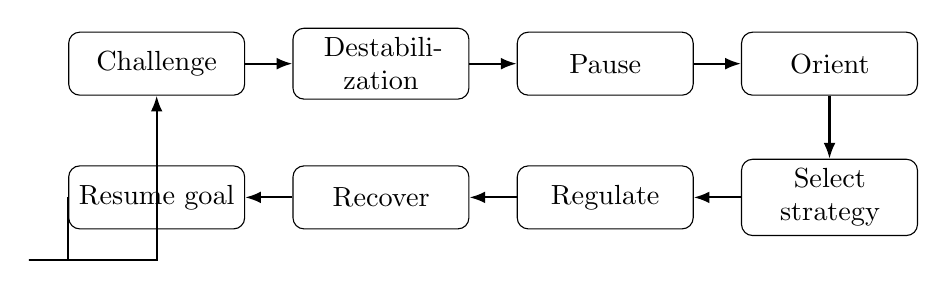
\begin{tikzpicture}[
node distance=8mm and 6mm,
box/.style={draw, rounded corners, align=center, minimum height=8mm, text width=2.0cm},
arrow/.style={-{Latex[length=2mm]}, thick}
]
\node[box] (challenge) {Challenge};
\node[box, right=of challenge] (destab) {Destabili-\\zation};
\node[box, right=of destab] (pause) {Pause};
\node[box, right=of pause] (orient) {Orient};
\node[box, below=of orient] (strategy) {Select strategy};
\node[box, left=of strategy] (regulate) {Regulate};
\node[box, left=of regulate] (recover) {Recover};
\node[box, left=of recover] (resume) {Resume goal};

\draw[arrow] (challenge) -- (destab);
\draw[arrow] (destab) -- (pause);
\draw[arrow] (pause) -- (orient);
\draw[arrow] (orient) -- (strategy);
\draw[arrow] (strategy) -- (regulate);
\draw[arrow] (regulate) -- (recover);
\draw[arrow] (recover) -- (resume);
\draw[arrow] (resume.west) |- ++(-5mm,-8mm) -| (challenge.south);
\end{tikzpicture}
\caption{Core ARC-ADHD regulation loop. A successful episode may contain destabilization or error; the target is recovery and return to the interrupted goal.}
\label{fig:closed-loop}
\end{figure}


The target is not continuous calmness or absence of negative affect. The target is context-appropriate recovery to goal-directed behavior following a bounded perturbation.

\subsection{Latent state and observed proxies}

Let the latent functional state be

\[
\mathbf{x}_t =
\begin{bmatrix}
E_t & R_t & B_t
\end{bmatrix}^{\mathsf T},
\]

where \(E_t\) denotes executive-control capability relevant to the current task, \(R_t\) denotes regulation-and-recovery capability, and \(B_t\) denotes body-state awareness relevant to strategy selection. These quantities are theoretical constructs and are not interpreted as stable clinical traits from a game session.

The controller observes only proxies,

\[
\mathbf{o}_t =
\left[
\mathbf{P}_t,
\mathbf{T}_t,
\mathbf{I}_t,
\mathbf{S}^{self}_t,
\mathbf{S}^{sens}_t,
\mathbf{C}_t
\right],
\]

where \(\mathbf{P}_t\) contains task-performance features, \(\mathbf{T}_t\) touchscreen features, \(\mathbf{I}_t\) optional low-burden inertial summaries, \(\mathbf{S}^{self}_t\) explicit child input, \(\mathbf{S}^{sens}_t\) tolerability or sensory-load indicators, and \(\mathbf{C}_t\) task context.

The intervention action is

\[
\mathbf{a}_t =
\left[
D_t,
L_t,
G_t,
Q_t
\right],
\]

where \(D_t\) is cognitive difficulty, \(L_t\) is sensory complexity, \(G_t\) is instructional guidance, and \(Q_t\) is regulation support.

\subsection{Bounded adaptive policy}

Adaptation is constrained by a prespecified safe action space:

\[
\mathbf{a}_{t+1} =
\Pi_{\mathcal{A}_{safe}}
\left[
\pi_{\theta}\left(\mathbf{o}_{t-k:t},\mathbf{a}_t\right)
\right].
\]

Safety rules and explicit child requests take priority over passive inference. Sensory overload is addressed before poor performance is interpreted as insufficient cognitive capacity. Thus \(D_t\) and \(L_t\) remain separable control variables.

\subsection{Operational definition of recovery}

For the first Signal Gate implementation, the pre-Phase 0 feature space is deliberately small. Rather than entering multiple redundant recodings of the same response event, the candidate definition contains one mandatory behavioral feature and two optional timing features.

The behavioral feature \(B\) is balanced rule success. If \(\tilde p_G\) is the Jeffreys-smoothed probability of a correct response on GO trials and \(\tilde p_N\) is the corresponding probability of a correct withhold on NO-GO trials, then

\[
B(t)
=
\frac{1}{2}
\left[
\tilde p_G(t)+\tilde p_N(t)
\right].
\]

Equal conditional weighting prevents the configured GO/NO-GO frequency from changing the interpretation of the behavioral component. Accuracy, commission errors, omissions, and rule-error rate remain available as descriptive telemetry but are not entered as separate equally weighted recovery dimensions.

The immediate preswitch reference and the recovery-score reference have different roles. The immediate current-rule window determines whether a challenge is eligible, but it does not normalize post-switch recovery. Because A\(\leftrightarrow\)B switching changes the response mapping, each rule has a stable reference collected in \texttt{RULE\_CALIBRATION}. For event \(e\) targeting rule \(r^\ast\), \(B_{\mathrm{ref},r^\ast}\) is computed from the calibration reference for that same rule and GO-stimulus identity.

The behavioral deficit is one-sided:

\[
d_B(t)
=
\max
\left[
0,
\frac{
B_{\mathrm{ref},r^\ast}-B(t)
}{
\max(s_{B,r^\ast}(t),\epsilon_B)
}
\right],
\]

where \(s_{B,r^\ast}(t)\) combines uncertainty in the target-rule Jeffreys-smoothed reference probabilities with the expected finite-window sampling variance under those reference probabilities. The observed postchallenge success rate is not used to enlarge its own denominator.

Two timing features are optional and use only correct GO trials from the same target-rule recovery reference. The immediate preswitch RT distribution is not used as a timing baseline. For target post-switch rule \(r^\ast\), let \(m_{\mathrm{ref},r^\ast}\) be the median correct-GO RT from the stable calibration block with the same rule and GO stimulus identity, and

\[
s_{\mathrm{RT},r^\ast}
=
\max
\left[
1.4826\,\mathrm{MAD}(RT_{\mathrm{ref},r^\ast}),
s_{\mathrm{device}}
\right],
\]

where \(s_{\mathrm{device}}\) is the timing floor from the qualified device profile. The correct-response slowing deficit is

\[
d_S(t)
=
\max
\left[
0,
\frac{
\mathrm{median}(RT_t)-m_{\mathrm{ref},r^\ast}
}{
s_{\mathrm{RT},r^\ast}
}
\right],
\]

and the variability-increase deficit is

\[
d_V(t)
=
\max
\left[
0,
\frac{s_t}{s_{\mathrm{RT},r^\ast}}-1
\right],
\qquad
s_t=
\max
\left[
1.4826\,\mathrm{MAD}(RT_t),
s_{\mathrm{device}}
\right].
\]

Faster correct responses and reduced variability do not receive positive credit. For every included component \(j\), define

\[
z_j(t)=-d_j(t),
\qquad
d_j(t)\ge 0.
\]

The composite score is

\[
q_e(t)
=
\sum_j w_j z_j(t),
\qquad
\sum_j w_j=1,
\]

and therefore \(q_e(t)\le 0\). This non-compensatory construction prevents unusually good performance in one component from cancelling a persistent deficit in another component.

Before Phase 0, only four feature models are admissible:

\begin{enumerate}
\item \(B\): balanced rule success only, with weight 1.0;
\item \(B+S\): behavior and slowing, each with weight 0.5;
\item \(B+V\): behavior and variability increase, each with weight 0.5;
\item \(B+S+V\): behavior with weight 0.5 and the two timing components with weights 0.25 each.
\end{enumerate}

There is no timing-only recovery model. Timing-enriched candidates are computable only under a timing-qualified device/profile. The feature definitions, minimum trial counts, candidate weights, and model-selection gates are versioned before Phase 0.

Recovery is evaluated only after the regulation sequence enters \texttt{RECOVERY\_MONITORING}. Let \(t_e\) denote challenge onset, \(t_m^{(e)}\) recovery-monitoring onset, and \(u_{e,k}\) the timestamp of score update \(k\). Define

\[
k_e^\ast
=
\inf
\left\{
k:
q_{e,r}\ge-\delta
\text{ for }
r=k,\ldots,k+w-1
\right\},
\]

where \(w\) is the required number of consecutive qualifying score updates and the complete confirming run must be observed before the censoring boundary.

The primary performance-recovery latency is

\[
T_{\mathrm{rec}}^{(e)}
=
u_{e,k_e^\ast}-t_m^{(e)}.
\]

Two additional process times are retained:

\[
T_{\mathrm{pre}}^{(e)}
=
t_m^{(e)}-t_e,
\]

and

\[
T_{\mathrm{total}}^{(e)}
=
u_{e,k_e^\ast}-t_e
=
T_{\mathrm{pre}}^{(e)}+T_{\mathrm{rec}}^{(e)}.
\]

Thus \(T_{\mathrm{rec}}\) is anchored to the onset of measurable post-regulation task performance rather than challenge onset. \(T_{\mathrm{pre}}\) captures the challenge-to-monitoring interval, including the pause/orient/strategy sequence, while \(T_{\mathrm{total}}\) describes the complete challenge-to-stable-return cycle. This decomposition prevents a longer strategy from mechanically appearing as slower post-regulation performance recovery.

If no complete qualifying stability run is confirmed before \(t_m^{(e)}+c_e\), the primary \(T_{\mathrm{rec}}^{(e)}\) observation is right-censored at \(c_e\). Censoring is therefore anchored to recovery-monitoring onset, not challenge onset.

The initial candidate implementation uses two distinct 12-valid-trial references with different roles: an immediate current-rule eligibility window before a candidate challenge and a stable target-rule recovery reference collected during \texttt{RULE\_CALIBRATION}. Only the latter normalizes \(B\), \(S\), and \(V\). Recovery itself is evaluated with an 8-valid-trial rolling postchallenge window updated every valid trial. The 12/8 counts are explicit Phase 0 measurement hypotheses rather than established psychometric constants. The final feature model, \(\delta\), \(w\), \(c_e\), and window definitions are frozen before Phase 1 inferential use.

\subsection{Recovery measurement-context invariance}

Recovery latency is interpretable only if improved post-challenge performance is not produced by changing the measurement conditions during the same event. On entry to recovery monitoring, the study therefore instantiates a versioned measurement context

\[
\mathbf{m}_e =
\left[
R_e,
D_e,
L_e,
W_e,
P_e,
C_e
\right],
\]

where \(R_e\) is the active task rule, \(D_e\) the cognitive-difficulty state, \(L_e\) the sensory configuration, \(W_e\) the response-window/timing configuration, \(P_e\) the stimulus-distribution specification, and \(C_e\) any prespecified cue assignment relevant to the event. Ordinary adaptive changes to these quantities are suspended until the recovery event is closed.

For a primary recovery record to remain scientifically valid, \(\mathbf{m}_e\) must remain unchanged throughout the recovery-assessment interval. A safety override, explicit child request, technical interruption, or other necessary action always takes priority over measurement. If such an action changes a score-relevant measurement condition before event closure, the event is recorded as recovery-data-invalid rather than as observed recovery or ordinary right-censoring. Adaptation may resume after the event has been closed and the goal state is restored.

A randomized cue can remain part of the recovery contrast when its assignment is made prospectively, represented in \(\mathbf{m}_e\), and held fixed according to the preregistered event definition. This rule prevents the controller from manufacturing apparently faster recovery by making the task easier, lengthening the response window, or otherwise changing the criterion environment after a difficult challenge.

\subsection{Calibration without outcome-driven tuning}

Phase 0 calibration is a measurement-engineering exercise rather than optimization against clinical response. Candidate feature models are evaluated using prespecified computability, reference-scale, timing-coverage, and leave-one-trial robustness criteria. The robustness test is applied across the complete preregistered neighborhood

\[
\delta \in \{0.25,0.50,0.75\}
\]

and stability windows of two or three consecutive score updates. The worst terminal-state flip fraction across this grid is used for the robustness gate; a model cannot be rescued by choosing the threshold pair that makes it appear stable.

The feature-model decision is explicitly parsimonious. If behavior-only \(B\) satisfies all hard measurement gates, it is retained unless a prespecified measurement failure requires an enriched model and that enriched model resolves the failure. If \(B\) fails and multiple enriched candidates pass, the lowest-complexity candidate is preferred; equal-complexity candidates are ordered by feature missingness and perturbation instability rather than clinical association.

Raw \(q\), median \(T_{\mathrm{rec}}\), and censoring proportion are reported as diagnostics but are not feature-selection targets, because their scales differ across candidate models and can be shifted by the score definition. External symptom, EDI, caregiver, teacher, functional, or treatment-group outcomes must not be used to choose the recovery definition. Once the Phase 0 measurement criteria are satisfied, the selected model, feature definitions, weights, window rules, final \(\delta\), stability window, censoring limit, missing-feature policy, and implementation version are locked before Phase 1 inferential use.

\subsection{Transfer hierarchy}

Evidence is classified into four levels:

\begin{enumerate}
\item trained-task learning;
\item proximal mechanistic change, such as reduced \(T_{\mathrm{rec}}\);
\item independent near transfer to an untrained executive task;
\item far transfer to externally assessed emotion regulation or everyday functioning.
\end{enumerate}

Clinical efficacy must not be inferred from Levels 1 or 2. A central falsification outcome is therefore substantial in-game improvement without corresponding independent change.

\section{Core Intervention Architecture}

ARC-ADHD is organized as one repeated regulation sequence rather than as a collection of unrelated minigames. A target session lasts approximately 15 to 20 minutes, with exact dose treated as a feasibility parameter.

\begin{figure}[htbp]
\centering
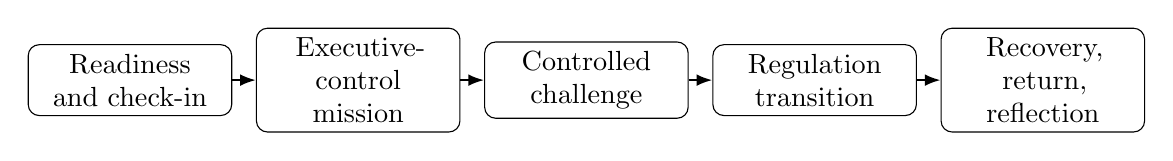
\begin{tikzpicture}[
node distance=3mm,
phase/.style={draw, rounded corners, align=center, minimum height=9mm, text width=2.35cm},
arrow/.style={-{Latex[length=2mm]}, thick}
]
\node[phase] (ready) {Readiness\\and check-in};
\node[phase, right=of ready] (exec) {Executive-control\\mission};
\node[phase, right=of exec] (challenge) {Controlled\\challenge};
\node[phase, right=of challenge] (reg) {Regulation\\transition};
\node[phase, right=of reg] (return) {Recovery, return,\\reflection};
\draw[arrow] (ready) -- (exec);
\draw[arrow] (exec) -- (challenge);
\draw[arrow] (challenge) -- (reg);
\draw[arrow] (reg) -- (return);
\end{tikzpicture}
\caption{Core session logic. Exact timings remain feasibility parameters, but challenge, regulation, and return are kept in a fixed causal order.}
\label{fig:session}
\end{figure}


\subsection{Readiness and calibration}

The application verifies the private phone's current BYOD qualification/capability profile, current sensory preferences, and whether the child wishes to use optional sound or haptics. A brief check-in captures subjective activation and any immediate reason to simplify or stop the session.

Before the first eligible rule-switch challenge, both Signal Gate rule mappings are exposed in a dedicated calibration state. This verifies that the child has encountered both mappings before switching is used as a perturbation. On timing-qualified execution profiles, calibration also supplies a correct-GO timing reference for each target rule and GO-stimulus mapping. Calibration trials are excluded from the recovery-event sample.

\subsection{Executive-control mission}

The minimum viable implementation requires at least one reproducible executive-control task that supports a stable baseline rule, bounded difficulty manipulation, identifiable challenge events, objective response accuracy and latency, and return to the same goal after regulation. Selective attention or inhibition with controlled rule switching is a suitable initial implementation because it can create recoverable perturbations without requiring a large content library.

\subsection{Controlled challenge}

The first Phase 0 operationalization uses one challenge family: an explicit Signal Gate rule switch from A to B or B to A. Other bounded perturbations remain possible later extensions but are not pooled into the initial recovery-measure stabilization sample.

Eligibility is evaluated before the switch and before any post-switch error, omission, slowing, or other apparent destabilization is observed. Thus the mechanistic event sample is not selected retrospectively on the basis of an unfavorable response. The eligibility contract requires an immediate current-rule reference, completed calibration of both mappings, no open recovery event, sufficient pacing and remaining event budget, healthy telemetry, and no active safety, overload, technical-interruption, or post-pause suppression state.

Core behavioral eligibility is distinguished from timing-feature eligibility. An otherwise valid event may contribute to the behavior-only recovery candidate when mobile timing is unqualified, whereas timing-enriched candidates additionally require a qualified timing profile and a target-rule/mapping-matched timing reference.

\subsection{Regulation transition}

The interface removes unnecessary stimulation and prompts a short sequence: pause, orient, choose one strategy, perform it, and return to the goal. Strategies may include paced breathing, muscle release, grounding, attentional redeployment, controlled movement, reappraisal, or simple problem solving. The intervention does not infer that one strategy is universally optimal.

\subsection{Recovery and return to goal}

The original objective resumes after regulation. Recovery is measured using the preregistered behavioral criterion rather than whether the first subsequent response is correct.

\subsection{Reflection and implementation intention}

At the end of the session the child briefly identifies which strategy was useful and connects it to an everyday situation using an implementation intention such as: if I notice \(X\), I will first do \(Y\), then return to \(Z\).

\subsection{Minimum sensory set}

Visual presentation is required for the ordinary task and instructions. Auditory cueing is optional and must not be required for successful completion. Haptic feedback is also optional and initially limited to a small standardized cue set, such as a pause/attention pattern. The intervention must remain usable when audio or haptics are disabled.

This requirement preserves accessibility and prevents sensory richness from being confused with the active treatment mechanism. Cognitive difficulty and sensory load therefore remain separate control variables.

\subsection{Minimal embodiment versus the separate embodied/AR study}

The core system may ask the child to notice breathing, tension, posture, contact with the floor or chair, or urge to move, and may use low-burden movement as part of a regulation strategy. These actions are part of strategy execution, not evidence that embodiment or AR causes transfer.

The separate embodied/AR paper manipulates physical movement and environmental coupling as independent variables. This boundary keeps the core causal claim focused on recovery training while preserving body orientation as a necessary part of some regulation strategies.

\subsection{Adaptation hierarchy}

The minimum controller hierarchy is: safety override; explicit child stop or difficulty request; sensory-overload rule; task-performance rule; recovery-state rule; scheduled research randomization; and ordinary progression. No passive sensor estimate may override an explicit child request or safety rule.

\subsection{Explicitly excluded core components}

The core MVP does not require front-camera adaptation, categorical emotion recognition, augmented-reality missions, spatial mapping, embodied movement as a transfer manipulation, alternating bilateral auditory stimulation, outdoor geolocation, or continuous raw audio/video recording. These exclusions are scientific boundaries rather than merely engineering deferrals.

\subsection{TIDieR implementation record}

For every research build, the intervention record should version: intervention name, rationale, software version, task materials, procedure, training or onboarding, delivery device, setting, session dose, tailoring rules, permitted modifications, and fidelity/telemetry checks \parencite{hoffmann2014tidier}. A frozen intervention manifest should be archived before the pilot randomized trial.


\subsection{Active-control boundary}

The active-control condition should use the same application shell and frozen BYOD compatibility policy where practical, with comparable session duration, device interaction, visual quality, neutral feedback, reward density, onboarding, and data-collection schedule. Its purpose is to control for nonspecific digital-game exposure, attention, novelty, expectancy, and study contact.

The control must not systematically reproduce the proposed active sequence. Specifically, it excludes controlled challenge followed by explicit pause--orient--strategy--regulate--recover training, recovery-state adaptation, individualized recovery feedback, and implementation-intention prompts linking the trained regulation sequence to everyday situations. If those elements are reproduced, the comparison no longer isolates the central ARC-ADHD mechanism.

Control credibility should be assessed without describing the condition to families as a placebo or inferior intervention. The software/configuration version, task list, reward configuration, sensory configuration, caregiver instructions, and deviations should be archived for both arms.

\section{Measurement Framework}

\subsection{Construct-to-measurement map}

Every claim must have a manipulable component, proximal observable, independent outcome, and falsification criterion.

\begingroup
\small
\setlength{\LTpre}{6pt}
\setlength{\LTpost}{6pt}
\renewcommand{\arraystretch}{1.1}
\begin{longtable}{p{2.7cm}p{3.2cm}p{3.2cm}p{3.2cm}}
\caption{Core construct-to-measurement map}\\
\toprule
Construct & Manipulation & Proximal measure & Independent test / falsifier \\

\midrule
\endfirsthead
\toprule
Construct & Manipulation & Proximal measure & Independent test / falsifier \\

\midrule
\endhead
\midrule
\endfoot
\bottomrule
\endlastfoot
Executive control & Rule load, inhibition, switching & Accuracy, latency, rule errors & Untrained executive task; no independent improvement weakens transfer claim \\
Recovery regulation & Controlled challenge plus strategy sequence & \(T_{\mathrm{rec}}\), unrecovered-event rate & External regulation/\allowbreak function measure; dissociation weakens mechanism claim \\
Multisensory cueing & Visual vs congruent added cue & Detection or inhibition under randomized eligible events & No proximal advantage implies cue can be simplified \\
Body orientation & Explicit check and strategy-linked bodily cue & Completion, self-report consistency & No relation to strategy use or recovery argues against retaining the prompt \\
\end{longtable}
\endgroup

\subsection{Core hypothesis-to-estimand map}

Table~\ref{tab:core-hypotheses} separates the prerequisite recovery-measurement gate from clinical, transfer, mechanistic, feasibility, and component-level claims. Companion-paper hypotheses on facial feedback, bilateral auditory stimulation, embodied/AR interaction, and wearable EEG are deliberately excluded.

\begingroup
\small
\setlength{\LTpre}{6pt}
\setlength{\LTpost}{6pt}
\renewcommand{\arraystretch}{1.1}
\begin{longtable}{p{0.8cm}p{2.5cm}p{2.5cm}p{2.5cm}p{3.0cm}}
\caption{Core hypotheses, estimands, outcomes, and falsification criteria}\label{tab:core-hypotheses}\\
\toprule
ID & Manipulation / contrast & Estimand & Outcome & Main falsifier \\

\midrule
\endfirsthead
\toprule
ID & Manipulation / contrast & Estimand & Outcome & Main falsifier \\

\midrule
\endhead
\midrule
\endfoot
\bottomrule
\endlastfoot
M0 & Four prespecified recovery-score candidates evaluated on eligible Phase 0 events & Measurement-gate metrics: computability, reference-scale floor use, leave-one-trial instability, and timing-qualified coverage & Candidate \(B\), \(B+S\), \(B+V\), and \(B+S+V\) definitions & No candidate passes all hard measurement gates; recovery measure must be redesigned rather than selected by clinical association \\
H1 & Core ARC-ADHD vs active control & Baseline-adjusted between-group post-intervention difference in the future confirmatory trial & Prespecified external regulation/\allowbreak dysregulation endpoint & No clinically meaningful advantage of the core condition in a sufficiently powered confirmatory trial \\
H2 & Core ARC-ADHD vs active control & Between-group change on an untrained executive assessment & Independent inhibition outcome; secondary flexibility outcome if frozen & Improvement restricted to Signal Gate or other trained tasks \\
H3 & Longitudinal change in recovery dynamics & Association between change in \(T_{\mathrm{rec}}\) and change in the external endpoint, adjusted for prespecified baseline factors & \(T_{\mathrm{rec}}\) and external regulation/\allowbreak function measure & Recovery telemetry changes without reproducible association with independent outcomes \\
H4 & Trained-task learning vs independent transfer & Difference in magnitude/pattern of improvement across outcome levels & Trained-task, near-transfer, and far-transfer outcomes & Treating large in-game gains as clinical efficacy when independent transfer is absent \\
H5 & Home-based delivery under the frozen BYOD policy & Feasibility proportions and uncertainty, not an efficacy effect & Recruitment, retention, dose, valid telemetry, overload, BYOD qualification/\allowbreak fallback & Prespecified red progression criteria or unresolved safety/\allowbreak measurement failure \\
H6 & Eligible cue event randomized among prespecified sensory conditions & Average proximal cue-condition effect among eligible events & Immediate detection/\allowbreak inhibition/\allowbreak recovery-related process measure & No proximal benefit or an unfavorable overload trade-off, supporting simplification \\
H7 & Configured body-orientation prompt within the regulation sequence & Prespecified association with strategy execution and subsequent recovery & Prompt completion, strategy use, recovery process & No reproducible relation to strategy use/\allowbreak recovery, arguing against retaining the prompt as an active mechanism \\
\end{longtable}
\endgroup

M0 is a measurement-validity gate, not a therapeutic hypothesis. It must be passed before \(T_{\mathrm{rec}}\) is used inferentially as a stable mechanistic quantity. H1 is a future confirmatory hypothesis, not a claim tested by Phase 0 or by the feasibility study. H5 is a progression hypothesis and must not be presented as evidence of efficacy. H6 and H7 are component-level mechanistic questions whose null results should simplify the intervention rather than be reinterpreted as support.

\subsection{Evidence ladder and inference gates}

ARC-ADHD uses four sequential evidence layers.

\begin{enumerate}
\item \textbf{Measurement validity:} the event definition, target-rule reference, recovery score, timing policy, missingness codes, and censoring rules are sufficiently stable and computable under the prespecified Phase 0 gates.
\item \textbf{Proximal mechanism change:} under a frozen measurement definition, the distribution of recovery outcomes changes in the prespecified direction across exposure or between randomized conditions.
\item \textbf{Independent transfer:} change is also observed on an assessment that does not reuse the trained task's stimuli, rule mapping, reward structure, or recovery calculation.
\item \textbf{Clinical/far-transfer effect:} a later adequately powered comparison shows a prespecified treatment effect on the frozen external endpoint.
\end{enumerate}

A favorable result at a later layer cannot repair failure of an earlier measurement layer. Conversely, passing measurement validity does not imply mechanism change, and mechanism change does not imply transfer or clinical efficacy. This ladder defines claim boundaries rather than a requirement that every development phase test all four layers simultaneously.

\subsection{Primary outcome candidate set}

The confirmatory primary endpoint is not yet frozen. The current audit identifies the Emotion Dysregulation Inventory (EDI) Reactivity score as the leading \emph{provisional} external endpoint for Phase 1/2 planning, conditional on a defensible Polish-language adaptation and validation pathway. This status is based on strong IRT-based psychometric evidence, demonstrated sensitivity to change, nationally representative youth evidence, and developmental coverage of the target age range \parencite{mazefsky2018edi,mazefsky2021edinational,kim2026edicommon}. The 2026 common-metric work explicitly links the EDI range of 6--17 years with the EDI-YC range of 2--5 years, strengthening developmental continuity without solving the Polish-localization question \parencite{kim2026edicommon}.

The Emotion Regulation Index for Children and Adolescents (ERICA) remains a scientifically relevant backup but its original validation is commonly reported for ages 9--16 and the current audit has not established a validated Polish pathway for the full ARC-ADHD age range. A contemporary evidence-base review rates ERICA more favorably than the older Emotion Regulation Checklist (ERC), while noting substantial limitations in the ERC evidence base \parencite{mazefsky2021measures}. BRIEF2 ERI remains a supporting candidate because the Polish Parent Form translation is officially listed, but its construct overlaps more strongly with executive functioning and Polish responsiveness evidence remains unresolved \parencite{jacobson2020brief2}. A CBCL-derived dysregulation profile remains useful as broad external corroboration but is intentionally transdiagnostic and less specific to the proposed regulation mechanism \parencite{peyre2015cbcldp}.

The provisional EDI choice does not authorize inferential use of an ad hoc Polish translation and does not constitute confirmatory endpoint lock. The choice between the 24-item Reactivity form and the 7-item Reactivity Short Form also remains explicitly unfrozen. Before participant-facing use, the exact EDI form/score, informant, Polish translation/adaptation method, scoring implementation, and evidence supporting longitudinal interpretation must be frozen.

The selection matrix must include:

\begin{enumerate}
\item construct match to the intended far-transfer claim;
\item validated age range for 8--12 years;
\item documented Polish-language adaptation and psychometric evidence;
\item licensing and administration burden;
\item caregiver, teacher, or self-report source;
\item reliability and expected floor/ceiling behavior;
\item evidence of responsiveness to change;
\item overlap with ADHD symptom content;
\item feasibility of blinded or independent administration.
\end{enumerate}

Until the Polish EDI pathway and confirmatory evidence package are complete, the paper continues to distinguish the provisional Phase 1/2 EDI Reactivity candidate from the formally unfrozen confirmatory primary endpoint.

\subsection{Secondary and mechanistic outcomes}

Secondary outcomes should include ADHD symptoms, functional impairment, quality of life, independent inhibition and working-memory measures, and acceptability/adherence. Teacher report is desirable when feasible because it reduces dependence on the same caregiver who observes intervention use.

Mechanistic outcomes include \(T_{\mathrm{rec}}\), unrecovered-event rate, challenge-specific error trajectories, strategy selection, sensory-overload events, pause frequency, and randomized cue effects.

\subsection{Expectancy and informant bias}

Because caregivers cannot be fully blinded to use of a game intervention, caregiver expectancy and credibility should be measured before meaningful exposure to the intervention and again if appropriate. The exact measure must be selected for suitability to caregiver-rated pediatric digital interventions rather than assumed valid by analogy with adult psychotherapy studies. Teacher or blinded assessor outcomes should be included where feasible.

\section{Staged Evaluation Programme}

The development programme is explicitly separated from a future confirmatory protocol. This sequencing is consistent with contemporary guidance for complex interventions, which emphasizes iterative development, explicit theory, context, stakeholder input, feasibility, and uncertainty before definitive evaluation \parencite{skivington2021complex}.

\begin{figure}[htbp]
\centering
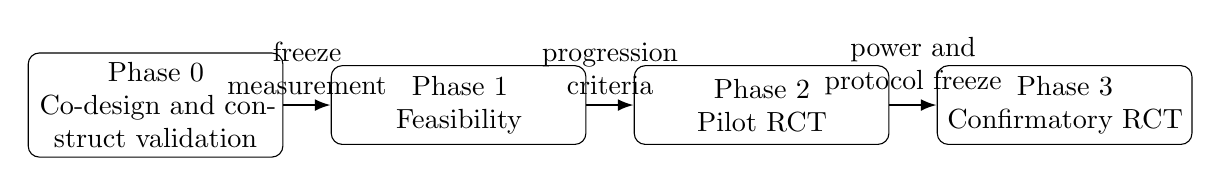
\begin{tikzpicture}[
node distance=6mm,
phase/.style={draw, rounded corners, align=center, minimum height=10mm, text width=3.0cm},
arrow/.style={-{Latex[length=2mm]}, thick}
]
\node[phase] (p0) {Phase 0\\Co-design and construct validation};
\node[phase, right=of p0] (p1) {Phase 1\\Feasibility};
\node[phase, right=of p1] (p2) {Phase 2\\Pilot RCT};
\node[phase, right=of p2] (p3) {Phase 3\\Confirmatory RCT};
\draw[arrow] (p0) -- node[above,align=center]{freeze\\measurement} (p1);
\draw[arrow] (p1) -- node[above,align=center]{progression\\criteria} (p2);
\draw[arrow] (p2) -- node[above,align=center]{power and\\protocol freeze} (p3);
\end{tikzpicture}
\caption{Staged research programme. The pilot estimates design parameters; the later confirmatory trial tests the frozen clinical hypothesis.}
\label{fig:programme}
\end{figure}


\subsection{Claim boundary by development stage}

The same numerical result has different meaning at different stages. Table~\ref{tab:stage-claims} defines the permitted claim boundary before describing each phase.

\begingroup
\small
\setlength{\LTpre}{6pt}
\setlength{\LTpost}{6pt}
\renewcommand{\arraystretch}{1.1}
\begin{longtable}{p{1.8cm}p{3.0cm}p{3.6cm}p{3.6cm}}
\caption{Permitted claims across ARC-ADHD development stages}\label{tab:stage-claims}\\
\toprule
Stage & Primary purpose & Claims permitted & Claims not permitted \\

\midrule
\endfirsthead
\toprule
Stage & Primary purpose & Claims permitted & Claims not permitted \\

\midrule
\endhead
\midrule
\endfoot
\bottomrule
\endlastfoot
Phase 0 & Co-design, construct operationalization, technical/safety validation & Comprehension, tolerability, measurability, telemetry validity, parameter stability, BYOD qualification feasibility & Clinical efficacy, superiority, therapeutic effectiveness \\
Phase 1 & Feasibility & Recruitment, retention, adherence, missingness, safety, recovery-distribution and implementation feasibility & Confirmatory treatment effect or proof of mechanism \\
Phase 2 & Pilot randomized trial & Effect/variance estimation, treatment separation, active-control response, missingness and design parameters for a definitive trial & Binary efficacy declaration based on nominal significance \\
Phase 3 & Confirmatory randomized trial & Prespecified causal treatment contrast on the frozen primary endpoint and prespecified secondary/mechanistic analyses & Post hoc endpoint substitution or reinterpretation of null primary results through exploratory outcomes \\
\end{longtable}
\endgroup

\subsection{Phase 0: co-design and construct validation}

Phase 0 evaluates comprehension, acceptability, challenge semantics, strategy prompts, sensory tolerability, and the stability of recovery-score construction. A provisional target of approximately 12--20 child-caregiver dyads can be used across iterative rounds, with stopping based on predefined design-coverage criteria and absence of new critical safety or comprehension failures across consecutive rounds rather than on efficacy statistics.

The first recovery-measure round restricts eligible mechanistic events to explicit Signal Gate A\(\leftrightarrow\)B rule switches. Both rule mappings are calibrated before eligible challenges, and challenge eligibility is decided before observing the post-switch response. Core event eligibility is recorded separately from timing-feature eligibility so that BYOD timing limitations remain observable rather than being hidden through post hoc event deletion. The pre-Phase 0 recovery feature space is restricted to \(B\), \(B+S\), \(B+V\), and \(B+S+V\), with model selection based only on prespecified measurement gates.

Clinical or developmental expertise must be represented in this phase. Collaboration should be substantive. Authorship is determined by contribution rather than added as a credibility device.

Key Phase 0 gates include whether at least 85\% of children can complete the challenge-regulation-recovery sequence after onboarding with no more than one neutral prompt, whether at least 90\% of eligible challenge events yield either a valid recovery time or an explicit right-censoring status, whether telemetry captures at least 95\% of required event fields, and whether the BYOD qualification/fallback process is operationally usable across the observed private-phone sample. These thresholds are project design targets rather than universal published cut-offs and must be ratified before the phase begins.

\subsection{Phase 1: feasibility}

A feasibility cohort of approximately 20--30 participants is intended to estimate recruitment, retention, completed dose, telemetry completeness, overload, adverse events, task comprehension, and the distribution/censoring of \(T_{\mathrm{rec}}\). This sample is not powered to establish efficacy.

Randomized pilot and feasibility guidance emphasizes that progression criteria should be prespecified and should address whether a future definitive trial can and should proceed, rather than whether a preliminary efficacy test is statistically significant \parencite{eldridge2016pilot,avery2017progression,mellor2021progression}.

The provisional traffic-light framework is summarized in Table~\ref{tab:progression}. The numerical values are intentionally conservative project targets selected to protect interpretability and participant burden. They must be reviewed by the clinical and statistical team before recruitment and cannot be relaxed after inspection of Phase 1 outcomes simply to permit progression.

\begingroup
\small
\setlength{\LTpre}{6pt}
\setlength{\LTpost}{6pt}
\renewcommand{\arraystretch}{1.1}
\begin{longtable}{p{3.0cm}p{3.0cm}p{3.0cm}p{3.0cm}}
\caption{Provisional Phase 1 progression criteria}\label{tab:progression}\\
\toprule
Domain & Green: go & Amber: amend & Red: stop/reconsider \\

\midrule
\endfirsthead
\toprule
Domain & Green: go & Amber: amend & Red: stop/reconsider \\

\midrule
\endhead
\midrule
\endfoot
\bottomrule
\endlastfoot
Recruitment & \(\geq 80\%\) of planned participants-per-site-per-month rate & 60--79\% & \(<60\%\) \\
Retention to post & \(\geq 80\%\) & 65--79\% & \(<65\%\) \\
Dose completion & \(\geq 75\%\) of participants complete \(\geq 75\%\) of sessions & 55--74\% meet dose & \(<55\%\) meet dose \\
Telemetry completeness & \(\geq 95\%\) of sessions complete for mechanistic fields & 85--94\% & \(<85\%\) \\
Valid recovery records & \(\geq 85\%\) of eligible events & 70--84\% & \(<70\%\) \\
Recovery censoring & \(\leq 25\%\) of eligible events & 26--40\% & \(>40\%\) \\
Overload termination & \(\leq 10\%\) of sessions & \(>10\)--20\% & \(>20\%\) \\
BYOD technical feasibility & Prespecified qualification target met; fallbacks and profile changes auditable & Target missed for a remediable device/OS subgroup & Compatibility or timing heterogeneity makes the planned mechanistic analysis uninterpretable \\
\end{longtable}
\endgroup

Any intervention-related serious adverse event or recurrent unmitigated safety pattern overrides the traffic-light table and triggers independent review.

\subsection{Phase 2: pilot randomized trial}

The pilot compares a frozen ARC-ADHD build with an active-control game while treatment as usual remains unchanged. Both arms use the same frozen BYOD compatibility policy and private-phone qualification procedure. The active control should match contact time, phone interaction, visual quality, reward density, and general engagement without reproducing the challenge-regulation-recovery sequence.

The pilot is designed to estimate recruitment under randomization, retention, missingness, outcome variance, baseline-follow-up correlation, active-control response, treatment separation, and effect uncertainty. It is not progressed because a nominal clinical \(p\)-value is favorable. Published sample-size guidance can inform the design, but no single rule such as a fixed number of participants per group is universally appropriate \parencite{whitehead2016pilot}.

\subsection{Phase 3: confirmatory randomized trial}

Only after the intervention, primary endpoint, active control, recovery definition, safety rules, and analysis plan are frozen should a confirmatory RCT be designed. Its sample size should be based on a prespecified minimally important effect, expected variance, repeated-measures correlation, attrition, and multiplicity strategy rather than the pilot point estimate alone.

The confirmatory protocol should be prospectively registered and reported according to SPIRIT 2025 \parencite{chan2025spirit}. The intervention description should satisfy TIDieR \parencite{hoffmann2014tidier}, and the completed randomized trial should be reported using CONSORT 2025 \parencite{hopewell2025consort}. Recruitment must not begin before applicable ethics approval and registration requirements are met.

\subsection{Polish implementation context}

The initial planned research setting is Poland. Recruitment sites, ethics-review body, validated Polish versions of all participant-facing measures, consent language, and data-controller responsibilities must be specified before the first participant is enrolled. Where a validated Polish instrument is unavailable, the project must not silently treat an ad hoc translation as equivalent to a validated measure.

\section{Statistical Framework and Telemetry}

\subsection{Analysis hierarchy}

The research programme separates measurement-validity estimands, feasibility estimands, mechanistic recovery estimands, independent near-transfer outcomes, and the future confirmatory far-transfer endpoint. A favorable result at a lower level does not substitute for evidence at a higher level, and an inferential recovery analysis is not interpreted before the recovery definition has passed its prespecified measurement gate.

\subsection{Analysis units and denominator contract}

ARC-ADHD uses different analysis units for different scientific questions. These denominators are defined prospectively and must not be exchanged after observing outcomes.

\begingroup
\small
\setlength{\LTpre}{6pt}
\setlength{\LTpost}{6pt}
\renewcommand{\arraystretch}{1.1}
\begin{longtable}{p{3.0cm}p{4.0cm}p{5.0cm}}
\caption{Primary analysis units and denominator rules}\\
\toprule
Analysis & Unit / denominator & Inclusion rule \\

\midrule
\endfirsthead
\toprule
Analysis & Unit / denominator & Inclusion rule \\

\midrule
\endhead
\midrule
\endfoot
\bottomrule
\endlastfoot
Challenge scheduling & Challenge candidate & Every candidate evaluated by the versioned eligibility rule, including suppressed candidates \\
Behavior-only recovery candidate \(B\) & Core-eligible rule-switch event & Every core-eligible event with scientifically valid behavioral recovery data; observed recovery and right-censored events remain in the time-to-event risk set \\
Timing-enriched recovery candidates & Timing-qualified core-eligible event & Prespecified subset of core-eligible events satisfying the frozen timing-profile and target-rule RT-reference requirements \\
Recovery-model validity & Candidate-specific eligible event & All events to which that candidate is prospectively applicable; computability failures remain visible in the denominator \\
Safety / tolerability & Participant and initiated session/event & All participants or sessions exposed to the relevant intervention component, regardless of recovery-data validity \\
Clinical / transfer outcomes & Randomized participant & Intention-to-treat population for randomized comparisons, with outcome-specific missing-data handling \\
\end{longtable}
\endgroup

A scientifically invalid recovery event is not ordinary right-censoring and does not remain in the primary recovery risk set after the invalidating context change. A telemetry-missing event is also distinct from a valid unrecovered event. Timing-unqualified events remain informative for the behavior-only candidate when its own requirements are satisfied; they must not be silently deleted from the behavioral denominator merely because \(S\) or \(V\) cannot be computed.

Candidate models can therefore have different applicable denominators during Phase 0. Any comparison of computability, instability, censoring, or latency must state the numerator, denominator, and reason for candidate-specific exclusion explicitly.

\subsection{Pilot clinical estimand}

The pilot randomized trial uses an intention-to-treat framework. The provisional clinical estimand is the between-group difference at post-intervention on the selected external regulation/dysregulation outcome, conditional on baseline value and prespecified design factors. Its purpose is to estimate direction, magnitude, confidence interval, variance, baseline-follow-up correlation, missingness, and parameters needed for the future confirmatory design rather than to make a binary efficacy declaration.

If baseline, post-intervention, and follow-up measurements are collected, a repeated-measures model can include treatment group, time, treatment-by-time interaction, and prespecified stratification variables. The covariance structure and handling of baseline must be frozen before the pilot database is locked.

\subsection{Independent near-transfer and functional outcomes}

Trained-task performance is separated from independent near transfer. The preferred inhibition candidate is a Stop-Signal Task implemented and analyzed according to consensus recommendations, including explicit data-quality checks and a prespecified SSRT estimation method \parencite{verbruggen2019stopsignal}. The assessment must use stimuli, response mapping, reward structure, and instructions that are independent of the trained Signal Gate task.

Because SSRT is timing sensitive, BYOD administration requires a qualified execution profile and prespecified handling of material phone/profile changes. If cross-device timing validation is inadequate, the task should be moved to a controlled assessment context rather than relaxing the measurement rules.

Everyday functional impairment is treated separately from ADHD symptoms and emotion dysregulation. WFIRS-P has published psychometric support in child/adolescent ADHD samples \parencite{gajria2015wfirs}, while the brief parent/teacher Impairment Rating Scale provides another validated child-ADHD impairment framework \parencite{fabiano2006irs}. Their use in the Polish study remains conditional on authorized Polish-language and licensing verification. The Polish SDQ can provide broad corroborating information, but existing Polish population work reported imperfect replication of the original subscale structure and called for further validation \parencite{mazur2007sdqpolish}. Therefore, SDQ is not treated as a substitute for a dedicated functional endpoint.

\subsection{Recovery-event analysis}

Event-level \(T_{\mathrm{rec}}\) is measured from entry into \texttt{RECOVERY\_MONITORING} to the first score update that begins a complete qualifying stability run. It is right-censored when no such run is fully confirmed within the monitoring censor window. Censored values must not be treated as ordinary maximum times. The challenge-to-monitoring interval \(T_{\mathrm{pre}}\) and total challenge-to-stable-return time \(T_{\mathrm{total}}=T_{\mathrm{pre}}+T_{\mathrm{rec}}\) are retained as separate process variables. This prevents strategy duration from being silently absorbed into the primary performance-recovery latency. Depending on the observed data-generating structure in feasibility work, a mixed-effects survival model, accelerated-failure-time model, or another preregistered time-to-event approach may be used. Participant, session, challenge direction, session number, and repeated events must be represented appropriately.

The primary values of \(\delta\), stability window \(w\), censoring limit \(c_e\), feature set, signs, and weights are frozen before pilot outcome inspection. A small preregistered grid around \(\delta\), \(w\), and \(c_e\) may be used for robustness analysis, but sensitivity analyses cannot replace the primary definition when the primary result is inconvenient.

During each recovery event, the score-relevant measurement context is also locked. Task rule, cognitive-difficulty state, sensory configuration, response-window timing, stimulus distribution, and any event-level cue assignment must remain at their prespecified recovery values until the event closes. A safety- or participant-driven change always takes priority, but if it changes the measurement context the event is classified as recovery-data-invalid rather than interpreted as faster recovery or ordinary right-censoring. The event record therefore distinguishes recovery validity from telemetry completeness.

\subsection{Randomized cue events}

Eligible cue events may be micro-randomized among visual-only, visual-plus-auditory, or visual-plus-haptic conditions when such a contrast is scientifically justified and safe. The proximal estimand is the average effect of assigned cue condition on a prespecified immediate outcome among events eligible for randomization.

The eligibility rule, randomization probability, carryover window, outcome window, repeated-event dependence, and missing-event handling must be preregistered. This component is mechanistic and does not create additional clinical primary endpoints.

\subsection{Missing data}

Missing external outcome data and censored recovery events are distinct problems. A participant with missing follow-up is not a censored recovery event, and a challenge event with corrupted telemetry is not treated as a child who failed to recover.

Missingness is reported by arm, time point, event type, and reason. If missing external primary-outcome data are material, the future confirmatory analysis should use a prespecified likelihood-based or multiple-imputation approach when its assumptions are plausible and should include sensitivity analysis to departures from the primary missing-data assumption.

\subsection{Telemetry specification}

The telemetry model is event based and versioned. At minimum, it records participant pseudonym, intervention version, schema version, session identifier, task/trial identifier, challenge-event identifier, challenge type, cognitive difficulty, sensory configuration, challenge onset, pre-challenge reference window, regulation actions, recovery parameters, recovery-monitoring onset, threshold-entry and confirmation timestamps, \(T_{\mathrm{pre}}\), \(T_{\mathrm{rec}}\), \(T_{\mathrm{total}}\) when observed, censoring status and reason, safety override, controller reason code, and missingness flags.

Within-session scientific timing uses a monotonic clock. Right-censoring and missingness have separate codes. Derived interpretable features are preferred over raw streams when raw data are not required by the scientific question.

Deterministic replay of the adaptive controller should be possible from the versioned configuration and logged inputs. The machine-readable recovery-event contract is maintained in the repository alongside the analysis specification.

\subsection{BYOD device heterogeneity}

The intervention is delivered on participant or caregiver private Android phones under a frozen compatibility policy. Qualification outcome, fallback use, coarse capability/performance class, and material device/profile changes are process variables rather than clinical endpoints.

When reaction-time-derived features contribute materially to a mechanistic analysis, the handling of capability class and device/profile changes must be prespecified. A material device change must not be treated as measurement continuity by default; timing-sensitive reference values may require reset, stratification, or sensitivity analysis. Exact manufacturer/model is not introduced post hoc as an unrestricted moderator merely because it is technically observable.

The programme also reports qualification, fallback, and nonqualification rates so that hardware-related exclusion is visible rather than hidden in recruitment loss.

\subsection{Mechanistic coherence is not causal mediation}

The core programme tests whether the proposed recovery process behaves coherently with the intervention theory, but it does not equate that test with proof of mediation. Evidence that ARC-ADHD changes \(T_{\mathrm{rec}}\), together with an association between change in \(T_{\mathrm{rec}}\) and an independent external outcome, supports the plausibility of the proposed mechanism. It does not by itself establish that recovery change causally transmits the intervention effect to the external outcome.

A formal mediation claim would require additional assumptions, a prospectively specified causal mediation estimand, appropriate temporal ordering, treatment of mediator--outcome confounding, and an analysis designed for that purpose. These requirements are outside the present framework unless they are added explicitly before data collection.

The programme therefore treats four patterns as scientifically distinct: improvement in both recovery and independent outcomes; improvement in recovery without independent transfer; independent improvement without detectable recovery change; and improvement restricted to trained-task performance. None of these patterns is reclassified post hoc as proof of the same mechanism.

\subsection{Multiplicity and claim hierarchy}

The research programme distinguishes one future confirmatory primary clinical endpoint from mechanistic and exploratory analyses. Optional companion modules have their own papers and do not enter the multiplicity family of the core trial unless they are explicitly integrated into a later confirmatory design.

Effect estimates should be reported with confidence intervals and clinically interpretable units. The analysis must not infer equivalence from a nonsignificant superiority test, select favorable recovery parameters after seeing the data, or interpret in-game improvement as a clinical endpoint.

\subsection{Intercurrent events and estimand sensitivity}

The confirmatory estimand must specify how treatment discontinuation, temporary interruption, rescue care, and technical non-delivery affect the target contrast. The preferred clinical policy estimand retains randomized participants regardless of adherence or intervention discontinuation, provided that the external outcome can be ascertained. A supplementary hypothetical estimand may address adequate intervention delivery, but it must not replace the randomized treatment-policy comparison.

For event-level recovery, interruption of the measurement context is not equivalent to discontinuation of the intervention. A safety override that changes the frozen recovery rule makes that event scientifically invalid for the latency endpoint, while remaining countable for safety and feasibility. Conversely, a valid event that reaches the prespecified monitoring limit without stable return is right-censored. The reason for every terminal state must be auditable.

\subsection{Dependence, informative observation, and robustness}

Recovery events are nested within sessions and participants. The number of eligible events may itself depend on previous performance, controller decisions, fatigue, or dropout. Therefore, an event-weighted average does not necessarily estimate the average child-level experience. The primary mechanistic analysis should define its weighting target prospectively, with participant-weighted summaries as a robustness check.

Potentially informative event availability and censoring will be characterized using prespecified predictors measured before the event. Sensitivity analyses may compare complete-event models with approaches that account for event selection or censoring, where identification assumptions are defensible. Such analyses are not presented as correcting unmeasured selection mechanisms.

Model diagnostics will assess time-to-event distributional assumptions, participant-level heterogeneity, influential clusters, and convergence. If proportional hazards assumptions are unsuitable, an accelerated-failure-time specification or restricted mean recovery-time contrast over a fixed horizon can be considered, with the selection rule determined before inferential outcome inspection. A restricted mean must account for right-censoring rather than substituting the censoring horizon as an observed recovery time.

\subsection{Interpretation under null and discordant findings}

A null difference in the external clinical endpoint cannot establish therapeutic equivalence or absence of any benefit. Similarly, a reduction in recovery latency without independent near or far transfer is evidence limited to the measured proximal process. If an optional sensor predicts recovery but fails to improve decisions under a prospective comparison, its incremental predictive value alone does not justify its deployment.

The interpretation will prioritize uncertainty intervals, feasibility limits, missingness, and measurement validity. Claims of clinical efficacy require the separately planned confirmatory evidence and cannot be inferred from engineering verification, simulation, or exploratory subgroup effects.

\section{Ethics, Data Governance, and Regulatory Boundaries}

\subsection{Research status and clinical oversight}

ARC-ADHD is a research prototype. It does not diagnose ADHD, replace established clinical care, or currently make a therapeutic product claim. The present paper does not state that ethics approval has been obtained. No child-participant recruitment should begin until the relevant Polish ethics-review process, institutional data-protection review, and study documentation are complete.

Clinical and developmental expertise is required before participant-facing phases. The project should involve clinicians or psychologists in construct validation, safety procedures, inclusion/exclusion criteria, adverse-event review, and interpretation. Authorship should follow actual scholarly contribution.

\subsection{Consent and assent}

Participation requires informed permission from the parent or legal guardian and age-appropriate assent from the child. Refusal or withdrawal by the child must stop research procedures even when parental permission exists, subject to applicable legal and ethics requirements.

Nonessential modules must use separable consent choices where scientifically feasible. In particular, the facial-feedback companion study uses a distinct opt-in rather than making camera processing a condition for access to the core intervention.

\subsection{GDPR and data minimization}

The project is designed in the European context and must comply with the General Data Protection Regulation and applicable Polish law. ADHD diagnosis and study variables that reveal mental or physical health status can constitute data concerning health. Biometric data receive special treatment under the GDPR when processed for the purpose of uniquely identifying a person. The ARC-ADHD programme therefore does not use facial processing for identity recognition and must not imply that every facial landmark is automatically an identification biometric \parencite{eu2016gdpr}.

The data-protection impact assessment, lawful basis, Article 9 condition where applicable, retention schedule, pseudonymization procedure, access control, processor agreements, and withdrawal/deletion procedures must be specified with the institutional data protection officer before data collection.

\subsection{Digital inclusion and private-device heterogeneity}

The programme deliberately adopts bring-your-own-device delivery from Phase 0. This improves ecological realism and avoids dependence on a dedicated study handset, but it makes hardware compatibility and access part of the feasibility question rather than eliminating them by design. The study therefore uses a frozen compatibility policy, on-device qualification, privacy-minimized capability profiling, fallbacks for optional modalities, and explicit requalification after material device or operating-system changes.

The proportion of screened private phones that are fully qualified, qualified with fallbacks, or not qualified should be reported. Nonqualification reasons and coarse capability/performance classes should be monitored for systematic exclusion. Device serial numbers, IMEI, Android identifiers, advertising identifiers, account identifiers, installed-app lists, precise location, and unrelated personal media are not required for the core research record. Timing-sensitive outcomes must be interpreted with explicit attention to device/profile changes rather than assuming identical measurement properties across private phones.

\subsection{Regulatory boundary}

Software may fall within the European medical-device framework depending on its intended purpose. The present research framework therefore avoids assuming either that ARC-ADHD is a medical device or that it is outside the MDR. Classification should be assessed when the intended purpose and product claims are fixed \parencite{eu2017mdr}.

Likewise, use of adaptive algorithms does not automatically make ARC-ADHD a high-risk AI system. Under the EU AI Act, classification depends on the intended use and, for product-linked systems, on conditions including whether the AI is a safety component or regulated product subject to the relevant conformity-assessment pathway \parencite{eu2024aiact}. Regulatory analysis must therefore follow the eventual deployed functionality rather than the research label.

\subsection{Safety and engagement}

The core application contains no advertising, loot boxes, streak-loss penalties, coercive engagement mechanics, or dark patterns. Explicit discomfort, overload, repeated failure, or safety events trigger simplification or termination of the current challenge. The adaptive controller logs why each high-level change occurred.

\section{Discussion}

The revised ARC-ADHD framework makes a narrower claim than the earlier integrated concept. It does not claim that adding more sensors, movement, AR, facial analysis, or unusual auditory stimulation should improve outcomes. Its central proposition is that repeated practice of a stable challenge-regulation-recovery rule can be measured within a digital intervention and can be tested for transfer beyond the trained task.

The strongest alternative explanation is engagement. A structured game may simply increase motivation or practice time without changing a transferable regulation process. Matching reward density, device exposure, contact time, and general visual quality in the active control is therefore essential. A second explanation is task familiarity: recovery may appear faster because the child learns the challenge sequence. Challenge-type variation, independent outcomes, and a confirmatory external endpoint are required to distinguish this from the proposed mechanism.

A third limitation is informant expectancy. Caregivers may observe the child using the intervention and may expect improvement. This can influence a caregiver-rated primary outcome even when the game has no specific regulation effect. Expectancy measurement, teacher report where feasible, and blinded independent assessment of selected outcomes should therefore be incorporated into later trials.

The framework is currently conceptual. No pilot or co-design data are presented. Statements about feasibility, acceptability, tolerability, and likely adherence are therefore hypotheses and development targets, not empirical findings. The one-author status of the current draft also limits the breadth of clinical and psychometric expertise represented. These limitations should be resolved through substantive collaboration before a participant-facing protocol is frozen.

The proposed mechanism also has an identification limit. A shorter \(T_{\mathrm{rec}}\) after repeated exposure would show change in the prespecified proximal process, and an association between recovery change and an independent outcome would support mechanistic coherence. Neither result alone proves causal mediation. A participant may improve on an external outcome through another pathway, or recovery telemetry may improve without transferable benefit. The statistical framework therefore treats proximal change, independent transfer, and a later confirmatory treatment effect as distinct empirical results rather than interchangeable evidence for one causal explanation.

Two design choices reduce avoidable measurement confounding without establishing construct validity by themselves. First, post-switch \(B\), \(S\), and \(V\) are normalized to a stable reference collected under the same target rule and GO-stimulus mapping rather than to the immediately preceding opposite rule. Second, \(T_{\mathrm{rec}}\) begins only when post-regulation recovery monitoring starts, while challenge-to-monitoring time \(T_{\mathrm{pre}}\) and total challenge-to-return time \(T_{\mathrm{total}}\) are retained separately. The remaining limitation is reference drift: an immutable within-session calibration reference may become less representative as practice or fatigue develops. Phase 0 must therefore quantify rule-specific reference stability across event order rather than silently refresh the baseline after seeing performance.

Bring-your-own-device delivery introduces a deliberate trade-off between ecological implementation and measurement control. Private-phone use can test whether the intervention is deployable under realistic hardware heterogeneity, but timing-sensitive measures may become less comparable across devices or after a device/profile change. Qualification, requalification, benchmark thresholds, coarse capability classes, and prespecified handling of timing discontinuities are consequently part of the measurement model rather than only software-engineering details.

Splitting the broader ARC-ADHD concept into companion studies is methodologically advantageous. Facial behavior has a distinct measurement-validity and privacy problem. Bilateral auditory stimulation has a distinct proof-of-mechanism problem. Embodied and AR interaction has distinct movement, spatial, device, and safety confounds. Wearable EEG has a separate acquisition, synchronization, artifact-control, and incremental-information problem. Treating these as separate causal or measurement questions makes null results interpretable and prevents feature accumulation from obscuring the primary mechanism.

The main unresolved measurement decision is the external primary endpoint. Candidate instruments differ materially in construct breadth, informant source, licensing, cultural adaptation, and overlap with ADHD symptoms. The endpoint should therefore be selected through a documented measurement audit rather than convenience.

Finally, \(T_{\mathrm{rec}}\) is useful only if its construction is reproducible. The feature set, reference window, stability criterion, and censoring rule cannot remain flexible after outcome inspection. The development programme explicitly treats those quantities as parameters that must be stabilized and frozen before inferential use. The accompanying supplementary methods specification extends this principle to the intervention manifest, challenge eligibility, controller replay, BYOD qualification, safety configuration, statistical analysis plan, and deviation record so that a later empirical report can be traced to a specific executable research state.

\section{Conclusions}

ARC-ADHD is reframed as a closed-loop research framework for training and measuring recovery to goal-directed behavior after controlled challenge in children with ADHD. The core paper separates the principal regulation mechanism from four optional companion lines: facial-behavior feedback, bilateral auditory stimulation, embodied/AR context transfer, and wearable EEG measurement.

The empirical sequence is deliberately conservative. First establish that the challenge-regulation-recovery cycle is understandable and safe and that the recovery measure itself passes prespecified validity and robustness gates. Then determine feasibility and estimate design parameters. Only after the intervention, primary endpoint, active control, recovery definition, safety rules, and analysis plan are frozen should a confirmatory trial test far-transfer efficacy.

The framework is weakened by outcomes such as improvement confined to trained tasks, unstable recovery metrics, recovery change without reproducible independent transfer, external improvement without detectable change in the proposed recovery process, no clinically meaningful advantage over active control on the future primary endpoint, or unacceptable burden. These patterns are informative outcomes rather than reasons to protect the model by adding further technology. Association between change in recovery and change in an external outcome is treated as mechanistic coherence, not as proof of causal mediation.

The immediate development gates are now more specific. The project must execute the Polish EDI localization and validation pathway before inferential use; stabilize and freeze eligible-challenge and \(q_e(t)\)/\(T_{\mathrm{rec}}\) definitions without clinical-outcome-driven tuning; complete real-device BYOD benchmarking and freeze the supported Android/runtime policy; freeze the first Signal Gate task, child-facing strategy wording, and safety/overload rules; and complete the named clinical, statistical, measurement, safety, privacy, and data-governance roles required before recruitment. These gates define what must be resolved before the conceptual framework can become a participant-facing empirical study.

\section{Transparency and Assistance Disclosure}

This manuscript is a conceptual and methodological research framework. It reports no participant data.

AI-assisted tools have been used during iterative drafting, editing, code support, and literature-discovery workflows. Human authors remain responsible for the scientific claims, source verification, wording, analysis plan, and final submitted content. Any journal submission should adapt this disclosure to the target journal's policy and should identify the tools and purposes required by that policy. Current ICMJE recommendations require transparent disclosure of AI-assisted technologies used in manuscript production and do not permit such tools to be listed as authors \parencite{icmje2026ai}.

Bibliographic records, especially recent publications, must be verified against publisher or indexing metadata before submission. No reference should be retained solely because it was suggested by an automated system.


\printbibliography[title={References}]
\end{document}
